\xchapter{Resultados}{} %sem preambulo
\label{cap-resultados}
% É recomendável utilizar `\acresetall' no início de cada capítulo para reiníciar o contator de referências às siglas.
\acresetall

O objetivo deste capítulo é apresentar os resultados das experiências
mencionadas no Capítulo~\ref{cap-experiencia} para discutir as
hipóteses de estudo.
Os resultados são apresentados em forma de gráficos que apresentam
breve discussões sobre detalhes percebidos durante as análises.

Todas os dados são recebidos em formulários
disponibilizados para os participantes no ambiente virtual.
No ambiente virtual foi escolhida a opção de não
obter registro do participante nos formulários, desta forma,
está garantido o anonimato das respostas.

Os dados recebidos não foram processados ou analisados
tempestivamente, assim, está garantido que não foram
realizadas mudanças na condução da metodologia
por influências dos dados em pesquisa.

Importante em pesquisa científica, a assinatura do termo
de consentimento livre e esclarecido pelos participantes foi digital,
isto é, assinado no ambiente virtual.
O termo utilizado está disponível no Apêndice~\ref{termo-ciencia}.

Além de facilitar o pós-processamento dos dados, a opção de
formulário digital em contrapartida a formulário impresso, foi
realizada com o objetivo de dissociar para o participante
uma falsa impressão de obrigatoriedade em participar do experimento,
que pode ocorrer com a utilização de formulário impresso disponibilizado
logo após a realização da atividade.


Uma vez registrados no ambiente virtual, durante o processo de análise de dados,
estes dados consolidadas foram extraídos e processadas com scripts de filtragem
e manipulação de dados\footnote{C, Bash e GnuPlot}, desta forma, foram consolidadas em informações que estão
apresentadas e serão discutidas neste capítulo.

As Seções~\ref{form-percepcoes} e \ref{form-disciplinas} descrevem
o conteúdo dos formulários apresentados aos participantes para obter
informações sobre as percepções destes;
a Seção~\ref{sec-ref-graficos} apresenta considerações relevantes para o
entendimento dos gráficos e demais informações apresentadas neste capítulo;
as Seções ~\ref{sec-sem-2016} e~\ref{sec-sem-2017}
apresenta os resultados para o semestre 2016.1 e 2017.1, respectivamente;
e, por fim, a Seção~\ref{sec-consideracoes-resultados} apresenta
considerações referente aos resultados onde serão discutidas
as hipóteses deste estudo.

\section{Formulário de percepções de problema}
\label{form-percepcoes}
Para cada problema os estudantes foram convidados a responder um formulário de percepções de problema.
Neste formulário foram apresentadas 32 questões aos participantes.
As cinco primeiras questões neste formulário foram de caracterização de perfil, como
idade e sexo.
As próximas vinte e quatro questões foram sobre as percepções dos participantes sobre a abordagem, o
problema, o tutor e auto avaliação.

Cada pergunta apresentou uma afirmação sobre o tema ao qual se desejava obter informações sobre as
percepções dos participantes.
A resposta do participante foi obtida em uma escala Likert com cinco itens, sendo as opções
``concordo'', ``concordo parcialmente'', ``indiferente'', ``discordo parcialmente'' e ``discordo''.

O participante também teve disponível um espaço aberto para incluir considareções adicionais sobre
as suas percepções sobre o problema especificamente e sobre a utilização da abordagem.

O questionário referente a percepção de participante sobre problema está disponível no
Apêndice~\ref{form-problema}.

\section{Formulário de percepções da disciplina}
\label{form-disciplinas}
Para obter as percepções da disciplina, os participantes foram caracterizados em \textit{desistente}
se por algum motivo desistiu da disciplina antes da conclusão, sendo assim, foi reprovado por
falta ou realizou trancamento, e \textit{concluinte} que concluiu a disciplina independente
de aprovação ou reprovação por conceito.

Aos participantes foi apresentado um formulário de acordo com a sua condição de desistente
ou concluinte.
Em ambos os casos o formulário apresentou 24 questões aos participantes.
O foco do formulário apresentado ao participante desistente é identificar indicações
sobre o motivo da desistência, enquanto para o participante concluinte o foco do
formulário apresentado está em identificar benefícios da abordagem na percepção
do participante.
As cinco primeiras questões neste formulário foram de caracterização de perfil, como
idade e sexo.
As próximas dezessete questões foram sobre as percepções dos participantes sobre referente
ao foco do formulário respondido.

Cada pergunta apresentou uma afirmação sobre o tema ao qual se desejava obter informações sobre as
percepções dos participantes.
A resposta do participante foi obtida em uma escala Likert com cinco itens, como as da Seção~\ref{form-percepcoes}.

O participante também teve disponível um espaço aberto para incluir considareções adicionais.

O questionário referente a percepção sobre disciplina de participante
concluinte está disponível no Apêndice~\ref{form-disciplina-concluinte}
e de participante desistente está disponível no
Apêndice~\ref{form-disciplina-desistente}.

\section{Considerações sobre os gráficos e resultados}
\label{sec-ref-graficos}
Para reduzir a quantidade de informações, por consequência melhor utilizar o
espaço, os gráficos utilizados nas seções que seguem neste capítulo
estão limpos de legendas.

Nas discussões apresentadas nas seções que seguem neste capítulo,
``participante'' está designando o estudante que respondeu a
pesquisa mencionada na discussão, não devendo ser confundido com
o estudante que participou da metodologia, uma vez que todos
os estudantes participaram da metodologia.


A Tabela~\ref{tabela-ref-graficos} apresenta o significado das barras
e a Figura~\ref{figura-ref-graficos} apresenta a legenda (cor da barra)
nos gráficos referentes as percepções dos participantes para as
afirmações mencionadas na Seção~\ref{form-percepcoes} sobre
o problema.
Um exemplo de leitura do gráfico é a barra \textbf{H} que apresenta
os resultados para a afirmação ``As situações abordadas pelo problema
se aproximam de um cenário real e atual.'', que deseja verificar
a percepção do participante se o problema apresenta realidade
e atualidade.

\begin{table}[h]
\caption{Referências para os gráficos}
\label{tabela-ref-graficos}
\begin{tabular}{c|p{14.6cm}}
Legenda & Pergunta respondida pelo participante \\
\hline
A & A construção da solução envolveu a elaboração, análise e exposição clara e racional de argumentos.\\
\hline
B & Foram identificadas ideias alternativas para uma mesma situação (ou seja, partes ou etapas individuais do problema).\\
\hline
C & Foram utilizadas, ao menos, uma das referências bibliográficas indicadas no texto do problema para estudo extraclasse.\\
\hline
D & Foi necessário recorrer a livros, vídeos, apostilas ou outros recursos não indicados no problema para chegar à solução.\\
\hline
E & O problema lhe deixou motivado para descobrir uma possível solução.\\
\hline
F & Você acredita que cumpriu com os objetivos de aprendizagem do problema.\\
\hline
G & Você teve que aprender novos conhecimentos (conceitos, habilidades ou atitudes) para chegar à solução do problema.\\
\hline
H & As situações abordadas pelo problema se aproximam de um cenário real e atual.\\
\hline
I & O conhecimento aprendido é útil para um profissional da área de Computação.\\
\hline
J & O texto do problema estava claro e bem escrito.\\
\hline
K & Havia no texto informações suficientes para direcionar a investigação.\\
\hline
L & O tempo disponibilizado para o desenvolvimento da solução foi adequado.\\
\hline
M & O problema estimulou o trabalho em grupo.\\
\hline
N & Você utilizou conhecimentos prévios (de um problema anterior ou mesmo de outro componente curricular) para chegar à solução do problema.\\
\hline
O & O problema exigiu o estudo individual de seus conteúdos fora das sessões tutoriais.\\
\hline
P & O método PBL me motiva para ir em busca do meu próprio conhecimento.\\
\hline
Q & As sessões tutoriais contribuem para o processo de resolução do problema.\\
\hline
R & Os participantes geralmente apresentam uma relação interpessoal boa e produtiva.\\
\hline
S & A quantidade de pessoas em cada Grupo Tutorial é apropriada.\\
\hline
T & Os problemas são úteis no processo de ensino-aprendizagem.\\
\hline
U & Os tutores contribuem, quando necessário, para a evolução das sessões tutoriais.\\
\hline
V & Os tutores deixam claros os critérios de avaliação do produto.\\
\hline
W & Os tutores dão feedbacks sobre o desempenho do grupo tutorial a cada sessão.\\
\hline
X & Eu gosto do método PBL.\\
\end{tabular}
\end{table}


A Tabela~\ref{tabela-ref-graficos2} e \ref{tabela-ref-graficos3} apresenta
o significado das barras nos gráficos referentes as percepções
dos participantres para as afirmações mencionadas
na Seção~\ref{form-disciplinas} sobre a aplicação da disciplina,
respectivamente para estudante \textit{concluinte} e \textit{desistente},
e a Figura~\ref{figura-ref-graficos} apresenta a legenda (cor da barra)
nestes gráficos.

\begin{figure}[!htb]
\centering
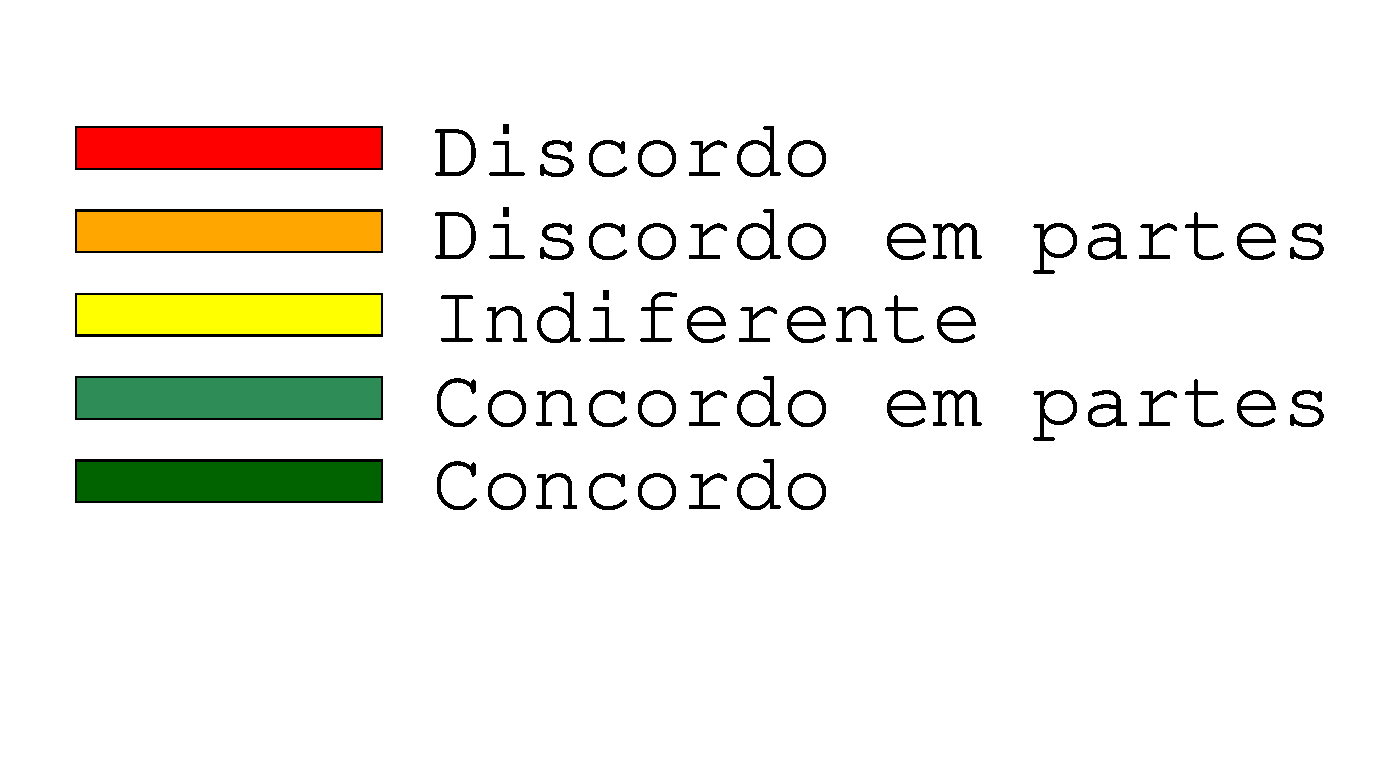
\includegraphics[scale=0.3,trim={0 4cm 0 1.5cm},clip]{figura-ref-graficos.eps}
\caption{Legenda para os gráficos em escala Likert} 
\label{figura-ref-graficos}
\end{figure}

\begin{table}[h]
\caption{Referências para os gráficos de percepção dos estudantes \textit{concluintes} sobre a disciplina}
\label{tabela-ref-graficos2}
\begin{tabular}{c|p{14.6cm}}
Legenda & Afirmativa respondida pelo participante \\
\hline
A & A metodologia da disciplina me agradou.\\
\hline
B & Gosto que a minha presença em sala faça parte da avaliação.\\
\hline
C & Gosto de ser avaliado pela participação durante as aulas.\\
\hline
D & Gosto de ter várias avaliações.\\
\hline
E & Gosto de avaliações em equipe.\\
\hline
F & Acredito que os tutores me motivaram suficientemente.\\
\hline
G & Consigo conciliar a disciplina com o trabalho profissional.\\
\hline
H & Eu entendi a metodologia PBL.\\
\hline
I & Falar em público é um grande problema para mim.\\
\hline
J & Eu gostaria de experimentar outras abordagens de ensino durante o meu curso além das aulas tradicionais.\\
\hline
K & A metodologia da disciplina me ajudou nas avaliações escritas (provas).\\
\hline
L & A metodologia da disciplina me ajudou a entender melhor a maioria dos conceitos estudados na disciplina.\\
\hline
M & A carga horária entre sessões tutorias e aulas expositivas foi suficientemente balanceada.\\
\hline
N & Tenho interesse em cursar outras disciplinas que possam utilizar esta abordagem.\\
\end{tabular}
\end{table}

\begin{table}[h]
\caption{Referências para os gráficos de percepção estudantes \textit{concluintes} sobre a disciplina}
\label{tabela-ref-graficos3}
\begin{tabular}{c|p{14.6cm}}
Legenda & Afirmativa respondida pelo participante \\
\hline
A & Desisti da disciplina porque a metodologia não me agradou.\\
\hline
B & Desisti da disciplina porque não gosto que a minha presença em sala faça parte da avaliação.\\
\hline
C & Desisti da disciplina porque não gosto de ser avaliado pela participação durante as aulas.\\
\hline
D & Desisti da disciplina porque não gosto de ter várias avaliações.\\
\hline
E & Desisti da disciplina porque não gosto de avaliações em equipe.\\
\hline
F & Desisti da disciplina porque acredito que os tutores não me motivaram suficientemente.\\
\hline
G & Desisti da disciplina porque não consigo conciliar a disciplina com o trabalho profissional.\\
\hline
G1 & Desisti da disciplina porque tive questões pessoais (exceto trabalho).\\
\hline
H & Eu entendi a metodologia PBL.\\
\hline
I & Falar em público é um grande problema para mim.\\
\hline
J & Eu gostaria de experimentar outras abordagens de ensino durante o meu curso além das aulas tradicionais.\\
\hline
N & Tenho interesse em cursar em breve a disciplina com esta abordagem.\\
\hline
M & Eu gostaria de experimentar a metodologia PBL, mas com mais carga horária de aulas expositivas.\\
\end{tabular}
\end{table}


Para cada um dos problemas foram construídos dois gráficos de resultados.
No primeiro gráfico são exibidos resultados para as respostas
dos participantes para questões afirmativas de percepção e
no segundo gráfico são exibidos os resultados para as notas atribuídas
ao problema pelo participante em uma avaliação geral.

Nos gráficos que seguem sobre as percepeções dos participantes para os
problemas e também sobre a disciplina, a disposição nas barras
foi construída para facilitar a leitura por nível de favorabilidade.
No caso de analisar os resultados em uma perspectiva mais conservadora
para a favorabilidade, é possível considerar que apenas a concordância
integral, isto é, o participante respondeu ``concordo'' para
a afirmação como favorável.
A inclusão de concordância em parte, isto é, também é considerado favorável que
o participante respondeu ``concordo em partes'' para a afirmação,
apresenta um resultado menos conservador em relação ao caso anterior.
E assim por diante, com a inclusão da resposta `indiferente'', que
representará o caso de favorabilidade onde não há discordância de alguma forma,
etc.

Ao longo da discussão, ao mencionar textualmente uma afirmativa de
algum dos formulários, foi incluído entre parêntesis a qual barra o texto
está se referindo, por exemplo, ``gosto da metologia PBL (X)''.

Para as conclusões apresentadas neste trabalho sobre percepção foi
considerada que uma afirmação obteve resultado positivo
se obteve $70\%$ de favorabilidade,
sendo favoráveis as percepções com algum nível de concordância,
isto é, o participante respondeu ``concordo''
ou ``concordo parcialmente''.

Nas seções a seguir que detalham os resultados, serão discutidos apenas os
pontos principais observados, positivos e negativos, em torno da
favorabilidade para o resultado positivo dentro dos critérios
definidos no parágrafo anterior.
A discordância integral nas afirmativas serão destacados para que
os possíveis pontos de melhoria estejam mais explicitados em meio
aos resultados positivos.

\section{Semestre 2016.1}
\label{sec-sem-2016}
\resultadoTurma{2016.1}{26}{9}{6}{57,7}{11}{8}{3}

\subsection{Problema 1 -- \ProblemaA}
\perfilProblema{\ProblemaA}{1}{2016.1}{14}
\perfilParticipante{27,9}{20}{51}{35,7}{71,4}{entre o terceiro e o quinto semestre}{}
\figuraPercepcaoParticipante{s1p1}{1}{2016.1}

É possível destacar que para todas as questões a favorabilidade
foi superior aos $70\%$. A favorabilidade foi superior aos $90\%$
para 12 afirmações apresentadas.
Apenas 6 afirmações receberam ao menos uma discordância integral.

A afirmação sobre ideias alternativas no caminho do problema (B)
foi a que teve a maior percepção de concordância por partes dos
participantes.
Entendemos que este resultado é explicado pelo problema
ter apresentado os conceitos de músicas, de forma que
os participantes precisaram realizar relacionamentos entre
os conceitos deste tema com os conceitos de linguagens
formais, e que os participantes perceberam que a depender do
nível de abstração poderá existir um caminho diferente.


A necessidade de recorrer aos materiais de apoio (D),
existência de informações suficientes no texto (K) e
sobre o participante gostar da metodologia baseada
em problemas (X) foram as afirmações com
as menores favorabilidades.
Embora possa parecer existir alguma contradição
sobre os resultados das duas primeiras, vale
ressaltar que os dados referente
a contribuição da sessão tutorial (Q) obtiveram
alta favorabilidade.

\figuraPercepcaoParticipanteNotas{s1p1}{1}{2016.1}{80}{5,00}{7,29}{quase}

\subsection{Problema 2 -- \ProblemaB}
\perfilProblema{\ProblemaB}{2}{2016.1}{12}
\perfilParticipante{28,5}{20}{51}{25,0}{75,0}{entre o terceiro e o quinto semestre}{}
\figuraPercepcaoParticipante{s1p2}{2}{2016.1}

Para 5 afirmações, na percepção dos estudantes, a favorabilidade foi integral.
Em 15 afirmações a favorabilidade superou os $90\%$.
Em apenas uma das afirmações a favorabilidade ficou pouco abaixo dos $70\%$, onde
$66,7\%$ dos participante acreditam que o problema estimulou
o trabalho em grupo (M).
Apenas 5 afirmações receberam ao menos uma discordância integral.

A contribuição dos tutores para a evolução do problema (U) foi a
afirmação melhor avaliada pelos participantes, assim como as demais
afirmações referentes aos tutores (W) e (V) também foram bem avaliadas,
indicando que os participantes aprovaram a participação
dos tutores na condução deste problema.

Para a construção do produto deste problema, os participantes
precisaram se reunir em equipe além das sessões tutoriais, desta forma,
acreditamos que as dificuldades referentes a se reunir fora das sessões tutorias
para trabalhar em grupo (M) estão também representados neste resultado.
Também observamos uma justificativa para este resultado ao analisar a favorabilidade para
a afirmação referente a percepção dos participantes com relação a quantidade
apropriada de estudantes em cada grupo tutorial (S).

\figuraPercepcaoParticipanteNotas{s1p2}{2}{2016.1}{70}{6,00}{7,17}{mais de}

\subsection{Problema 3 -- \ProblemaC}
\perfilProblema{\ProblemaC}{3}{2016.1}{8}
\perfilParticipante{31,4}{20}{51}{28,6}{85,7}{até o quinto semestre}{ para cada três participantes}
\figuraPercepcaoParticipante{s1p3}{3}{2016.1}

Para 7 afirmações, na percepção dos estudantes, a favorabilidade foi integral.
Em três afirmações a favorabilidade ficou abaixo dos $70\%$, mas apenas 2
afirmações receberam ao menos uma discordância integral.

A contribuição das sessões tutorias para o processo
de resolução do problema (Q) obteve a melhor avaliação pelos
participantes.
Entendemos que essa afirmação é bem avaliada sempre que
os participantes conseguem perceber uma informação de
grande relevância para a solução durante a sessão
tutorial, neste caso, a ideia de como manipular a pilha
de forma a manter a proporção exigida pelo problema
surgiu durante uma sessão tutorial.

No que diz respeito a quantidade de pessoas em
cada grupo tutorial (S) ser a afirmação a obter a pior
avaliação a justificativa pode ser obtida quando
é observada em conjunto com a afirmação referente ao
trabalho em equipe (M) que também esteve entre
as piores avaliações para este problema, neste caso,
ambos resultados são explicados pela quantidade de
participantes nas sessões tutoriais.

\figuraPercepcaoParticipanteNotas{s1p3}{3}{2016.1}{90}{6,00}{7,50}{quase}

\subsection{Problema 4 -- \ProblemaD}
\perfilProblema{\ProblemaD}{4}{2016.1}{8}
\perfilParticipante{31,5}{20}{51}{25,0}{87,5}{até o quinto semestre}{}
\figuraPercepcaoParticipante{s1p4}{4}{2016.1}

Para 12 afirmações, na percepção dos estudantes, a favorabilidade foi integral.
Em todas as afirmações a favorabilidade ficou acima dos $70\%$.
Em 4 afirmações foi recebida ao menos uma discordância integral.

A máquina de Turing foi o principal objetivo de aprendizagem para o Problema 4
aplicado no semestre 2016.1, sendo que para os participantes a afirmação
melhor avaliada diz respeito a utilidade dos conhecimentos aprendidos para 
o profissional da área de Computação (I).
Este problema foi muito bem avaliado pelos participantes para todas
as afirmações, mas cabe destacar os resultados para as afirmações que
dizem respeito a necessidade de aprender novos conhecimentos (G) e
motivação dos participantes para resolver o problema (E).

\figuraPercepcaoParticipanteNotas{s1p4}{4}{2016.1}{90}{5,00}{7,50}{quase}

\subsection{Problema 5 -- \ProblemaE}
\perfilProblema{\ProblemaE}{5}{2016.1}{7}
\perfilParticipante{32,3}{20}{51}{28,6}{71,4}{até o quinto semestre}{}
\figuraPercepcaoParticipante{s1p5}{5}{2016.1}

Para 6 afirmações, na percepção dos estudantes, a favorabilidade foi integral.
Em apenas duas afirmações a favorabilidade ficou abaixo dos $70\%$.
Em 9 afirmações foi recebida ao menos uma discordância integral, desta forma,
indicando vários pontos de atenção para a abordagem deste problema
em outras situações.

Este também foi um problema em que os participantes se reuniram em grupo para
construir uma solução, assim, como no Problema 2 no semestre 2016.1, a
afirmação pior avaliada também foi referente ao trabalho em equipe (M) que
indicamos que o resultado também inclui as dificuldades em se reunir além
das sessões tutoriais.

Ideias alternativas (B), utilização de referências bibliográficas (C),
recorrer a materiais não indicados nas referências (D), motivação
para resolver o problema (E), o tempo para resolução (L), a quantidade de
pessoas no grupo da sessão tutorial (S), utilidade do problema para o
processo de ensino e aprendizagem (T), \textit{feedback} dos
tutores (W), além da afirmação sobre o trabalho em equipe (M)
mencionado no parágrafo anterior, foram as afirmações com ao menos
uma discondância integral.
O mais possível é que este resultados sejam justificados pela sobrecarga
adicional que os estudantes possuem no fim do semestre, momento em que
este problema foi aplicado.
Ainda assim, não se deve desconsiderar que estes são pontos
de atenção claros, mas que mesmo em outras metodologias, com pesquisa
semelhante, os resultados da sobrecarga estariam também explicitados.

\figuraPercepcaoParticipanteNotasA{s1p5}{5}{2016.1}{70}{}{7,00}{pouco mais de}

\subsection{Percepção dos concluintes}

\subsection{Percepção dos desistentes}

\section{Semestre 2017.1}
\label{sec-sem-2017}
\resultadoTurma{2016.1}{50}{x}{y}{z}{a}{14}{b}


\subsection{Problema 1 -- \ProblemaG}
\label{sec-2017-p1}
\perfilProblema{\ProblemaG}{1}{2017.1}{12}
\perfilParticipante{26,1}{19}{44}{18,2}{72,7}
{até o terceiro semestre}{ para cada seis participantes}
\figuraPercepcaoParticipante{s2p1}{1}{2017.1}

Para 7 afirmações apresentadas a favorabilidade ficou um pouco abaixo dos $70\%$, mas
para 10 afirmações foi superior aos $90\%$.
Em 11 afirmações foi recebida ao menos uma discordância integral.

Neste problema com o objetivo de aprendizagem foi Linguagens
Formais, sendo consenso de percepção dos participantes que
este problema apresenta um conhecimento útil para um profissional
da área de Computação (I).

É possível destacar o excelente resultado para a afirmação que diz respeito a
utilidade do problema no processo de ensino e aprendizagem (T).
A explicação para este resultado está no fato de que os estudantes
conseguiram realizar bem as correlações entre os conceitos
do código Morse, apresentado no problema, com os conceitos de
linguagens formais, que são os objetivos de aprendizagem para
este problema.

Em uma análise mais detalhada dos dados foi possível
detectar que a discordância integral está concentrada
em 3 participantes, onde apenas um destes apresentou
5 discordâncias integrais.
Estes números além de indicar pontos possíveis de
priorização, também podem indicar a necessidade
de um nivelamento maior dos estudantes para a aplicação
da metodologia.

\figuraPercepcaoParticipanteNotas{s2p1}{1}{2017.1}{90}{5,00}{8,25}{quase}

\subsection{Problema 2 -- \ProblemaB}
\perfilProblema{\ProblemaB}{2}{2017.1}{13}
\perfilParticipanteA{24,3}{19}{38}{8,3}{63,6}
{até o terceiro semestre}{ quatro para cada dez}
\figuraPercepcaoParticipante{s2p2}{2}{2017.1}

A favorabilidade ficou um pouco abaixo dos $70\%$ em 6 afirmações apresentadas,
sendo superior aos $80\%$ em 12 afirmações.
Em 14 afirmações foi recebida ao menos uma discordância integral.

Neste problema o objetivo de aprendizagem principal foi
Autômatos Finitos, sendo consenso de percepção dos participantes que
este problema apresenta um conhecimento útil para um profissional
da área de Computação (I) e que é necessário aprender novos
conhecimentos (G).

Apenas um dos participantes respondeu com discordância integral para
8 afirmações, assim, também se faz necessário considerar a
necessidade de nivelamento do grupo, como mencionado
na Seção~\ref{sec-2017-p1}.

Apesar de obter favorabilidade muito próxima aos $70\%$, a afirmação
sobre o participante gostar da metodologia PBL (X) teve como
destaque negativo receber a maior discondância integral nessa
replicação.

\figuraPercepcaoParticipanteNotas{s2p2}{2}{2017.1}{60}{5,00}{7,31}{pouco mais de}

\subsection{Problema 3 -- \ProblemaC}
\perfilProblema{\ProblemaC}{3}{2017.1}{11}
\perfilParticipanteA{25,1}{19}{38}{0}{63,6}
{até o terceiro semestre}{ quatro para cada dez}
\figuraPercepcaoParticipante{s2p3}{3}{2017.1}

A favorabilidade ficou um pouco abaixo dos $70\%$ em apenas uma afirmação,
sendo superior aos $80\%$ para 21 destas afirmações.
Em apenas 2 afirmações foi recebida ao menos uma discordância integral.

Para este caso a percepção dos participantes
sobre a relevância das sessões tutorias no processo
de resolução do problema (Q), assim como no semestre
anterior, obteve favorabilidade integral, com o destaque de
que para este semestre todas as respostas recebidas foram de
total concordância.

A afirmativa pior avaliada diz respeito a percepção dos participantes
sobre o \textit{feedback} dos tutores a cada sessão tutorial (W).
Para este caso, apesar do resultado ainda ser alto, ficou como
um ponto de atenção aos tutores.

A Figura~\ref{aval-s2p3} apresenta o gráfico da
avaliação do participantes para o Problema 3 aplicado no semestre 2017.1.

\begin{figure}[!htb]
\centering
\includegraphics[scale=0.18]{notas-s2p3.eps}
\caption{Avaliação dos participantes do semestre 2017.1 para o Problema 3}
\label{aval-s2p3}
\end{figure}

Assim como no semestre anterior, este problema foi muito bem avaliado
pelos participantes, assim, todas as notas atribuídas foram maiores
ou iguais $7,00$ e uma média de $8,18$.

Entre os problemas que foram replicados em ambos os semestres, este
notadamente é o que apresentou as melhores avaliações pelos participantes
em todos os critérios, evidenciando o potencial da metodologia em uma
disciplina teórica com a utilização de um problema do ``mundo real''.

\subsection{Problema 4 -- \ProblemaD}
\perfilProblema{\ProblemaD}{4}{2017.1}{10}
\perfilParticipanteB{25,7}{19}{38}{11,1}{88,9}
{até o terceiro semestre}{igual}
\figuraPercepcaoParticipante{s2p4}{4}{2017.1}

Para todas as afirmativas a percepção dos participantes obteve favorabilidade
superior aos $70\%$. Em 5 afirmações foi recebida ao menos uma discordância
integral.

O destaque positivo para este problema foi a favorabilidade em relação
a necessidade de recorrer a materiais fora da bibliográfia básica (D).
Este é uma característica de estudo muito relevante no desenvolvimento
do estudante que passa a ver a necessidade de explorar fontes diversas
de informação para construir o seu conhecimento.

Como ponto de atenção, apesar de a favorabilidade ser igual aos $70\%$ para
a percepção do participante sobre a adequação do tempo disponível para desenvolver
a solução (L), houve uma quantidade relevante de discordância integral para esta afirmativa.

Este foi outro problema que foi bem avaliado em todos os critérios em ambos
os semestres.
\figuraPercepcaoParticipanteNotas{s2p4}{4}{2017.1}{80}{6,00}{7,31}{quase}

\subsection{Problema 5 -- \ProblemaE}
\perfilProblema{\ProblemaE}{5}{2017.1}{7}
\perfilParticipanteB{27,0}{20}{38}{20,0}{100,0}
{até o terceiro semestre}{semelhante}
\figuraPercepcaoParticipante{s2p5}{5}{2017.1}

Em 3 afirmações a favorabilidade ficou abaixo dos $70\%$ e 5 afirmações
receberam ao menos uma discordância integral.

Em contraste com o resultado que o mesmo problema teve com
os participantes do semestre 2016.1, onde foi a afirmação com a
pior favorabilidade, para os participantes neste semestre de
2017.1, a percepção de que o problema estimula o
trabalho em grupo (M) foi a afirmação melhor avaliada
para o Problema 5.
A diferença de resultado é justificada ao observar
a percepção dos participantes com relação a quantidade
apropriada de estudantes em cada grupo tutorial (S).

A afirmação com a menor favorabilidade diz respeito
a percepção de cumprimento dos objetivos de aprendizagem
pelo participante (F).
Neste ponto cabe destacar que ao apresentar um resultado
negativo para esta afirmação, uma vez que com outros
problemas dentro do mesmo grupo tiveram favorabilidade
melhores, se pode questionar o problema e não
a metodologia.
Também não se pode deixar de considerar o nível de abstração
mais elevado para o entendimento dos conceitos deste
problema em relação aos demais.

\figuraPercepcaoParticipanteNotas{s2p5}{5}{2017.1}{70}{5,00}{7,43}{pouco mais de}

\subsection{Percepção dos concluintes}
\figuraPercepcaoParticipanteDisciplina{concluintes-2017}{concluintes}{2017.1}

\subsection{Percepção dos desistentes}
\figuraPercepcaoParticipanteDisciplina{desistentes-2017}{desistentes}{2017.1}


\section{Considerações finais}
\label{sec-consideracoes-resultados}

Para responder as hipóteses as quais este estudo se propõe, utilizamos
os resultados apresentados neste capítulo.
